\chapter{Part 1: Synchronization of Extreme Events}
\label{c:event_sync}
During the primary monsoon season, floodings and landslides caused by extreme rainfall can lead to massive societal and environmental damage \citep{Stolbova.2015}. It is thus crucial to be able to analyze, detect and potentially predict such extreme rainfall events, especially as their proportion tends to further increase with global warming \citep{Stolbova.2015} [TODO: cite Goswami?].

A way of analysis that \citet{Stolbova.2015} has proposed is the computation of climate networks based on different locations in India, followed by an analysis of the resulting networks using graph centrality measures. We strongly base this chapter on her work and thus summarize her approach in \cref{sst:event_sync}. We also explain the network measures that will be applied to the resulting climate networks (\cref{sst:network_measures}) and introduce the dataset that will be used as a basis for all calculations (TRMM, \cref{sst:trmm_dataset}).

\cref{st:event_sync_implementation} then provides an overview of our approach to the creation of climate networks and explains where our approach differs from the work of \citep{Stolbova.2015}. Following up in \cref{st:event_sync_results}, we analyze and visualize the computed climate networks using graph centrality measures and try to interpret the results in contrast to the known factors of monsoon behavior. Concluding this chapter in \cref{st:event_sync_conclusion}, we elaborate the usefulness of our results and how they could be improved upon.

\section{Related Work}
[TODO: need text here?]

\subsection{The TRMM dataset}
\label{sst:trmm_dataset}
The Tropical Rainfall Measurement Mission (TRMM) is a precipitation research effort by the National Aeronautics and Space Administration (NASA) and the Japanese Aerospace Exploration Agency (JAXA). It is based on the TRMM observatory, a satellite that was launched into space on the 27th of November, 1997. The products based on TRMM range from the raw output of the multitude of sensors on the satellite to the highly aggregated and gridded rainfall estimates we will be using in this work \citep{GoddardEarthScienceDataInformationandServicesCenter.2016}.

More specifically, the TRMM product that we will be using is a 3-hourly estimate of surface rainfall aggregated from the satellite sensors in combination with surface gauge values and imagery from other satellites. This product is referred to as 3B42 or TMPA and is also available in a daily variation, where the eight 3-hourly measurements (i.e., 00:00, 03:00, 06:00 and so on) have been summed up to provide a single daily rainfall estimate.

[TODO: update coordinates and grid specifics] 3B42 is available for the area between 50\degree N. and 50\degree S. We subset this area to cover the entire Indian subcontinent (x-x\degree N, x-x\degree E). These border coordinates are a superset of the ones used in \citep{Stolbova.2015}: the grid has been extended  such that it can be cleanly aggregated from a 0.25\degree spatial resolution to the 0.75\degree resolution of the ERA-Interim dataset (which we will use later on). \cref{fig:trmm_area} shows the excerpt of the TRMM dataset that we will be using in this work.

\begin{figure}[h]
  \centering
  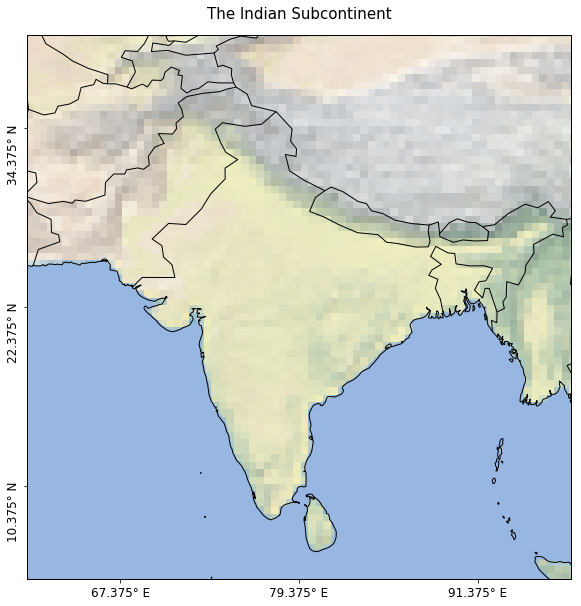
\includegraphics[width=0.5\linewidth]{./99_appendix/img/area_overview}
  \caption{The Indian subcontinent as extracted from TRMM.}
  \label{fig:trmm_area}
\end{figure}

The TRMM dataset is unique in that it offers very high-resolution precipitation estimates since January 1998. It can prove useful for research based on the distribution, frequency, and intensity of rainfall, i.e., for calculating extreme rainfall events \citep{Stolbova.2015}. However, it has to be taken into consideration that the TRMM products are based on complex algorithms and have been derived from different sensors and sources \citep{Huffman.2017b}.

After the TRMM satellite's fuel went low in 2014, it was decommissioned in April 2015 and re-entered earth's atmosphere in June 2015. The TMPA product is still being produced until 2018, albeit without the sensors of the TRMM observatory and with less accuracy \citep{Huffman.2017}.

Built on the success of the TRMM mission, NASA and JAXA have launched its successor GPM (Global Precipitation Measurement) in 2014 \citep{GoddardEarthScienceDataInformationandServicesCenter.2011}. However, as its data is only available starting from 2014, GPM is currently unsuitable for long-term precipitation research. TRMM or an alternative dataset are currently still needed but the updated algorithm developed for GPM will soon be applied to the existing TRMM data. The availability of reprocessed data back to 1998 can thus be expected in 2018 \citep{Huffman.2016}.


\subsection{Event synchronization \& climate networks}
\label{sst:event_sync}
The concept of event synchronization applied in \citet{Stolbova.2015} as well as in our work was first defined in \citet{QuianQuiroga.2002}. \citet{QuianQuiroga.2002} sought to develop a simple algorithm that could be applied to any two time series of events, resulting in a measure that defines the synchronization of said time series. Synchronization measures are generally related to standard measures like cross correlation. They can, however, convey more complex relationships due to their non-linearity \citep{QuianQuiroga.2002}.

\subsubsection{Basic event synchronization}
The basic principle of the event synchronization measure as found in \citet{QuianQuiroga.2002}, \citet{Malik.2010} and \citet{Stolbova.2015} is setup as follows: given the two time series $i$ and $j$ and their respective events $l$ and $m$ occuring at times $t^i_l$ and $t_j^y$, we measure the synchronicity for all possible pairs of events between both series. We classify events as synchronous if they occur closely simultaneous, i.e., within a certain range from each other. This allowed range of occurrence is called \textit{time lag} and is calculated by taking the minimum interevent distance $\tau^{ij}_{lm}$ like so\footnote{If event rates were fixed, a global time lag $\tau$ could be defined, greatly simplifying calculations.}:

\begin{equation}
\tau^{ij}_{lm} = 0.5 * min\left\{t^i_{l+1} - t^i_l, t^i_l - t^i_{l-1}, t^j_{m+1} - t^j_{m}, t^j_{m} - t^j_{m-1}\right\}
\end{equation}

The synchronicity $J$ of any two events $t_i^x$ and $t_j^y$ is then calculated as follows:

\begin{equation}
  J_{ij} =
  \begin{cases}
    1, & \text{if } 0<t^x_i-t^y_j\leq\tau_{ij}, \\
    0.5, & \text{if } t^x_i=t^y_j, \\
    0, & \text{else.}
  \end{cases}
\end{equation}

Applying this to the full time series $i$ and $j$, the number of synchronous events where an event in $i$ leads an event in $j$ is defined like:

\begin{equation}
  c(i \mid j) = \sum\limits^{s_i}_{l=1} \sum\limits^{s_j}_{m=1} J_{ij}
\end{equation}

The same formula applies to the reversed situation, i.e. $c(j \mid i)$, with $s_i$ and $s_j$ being the number of events in the respective time series. Combining the results of $c(i\mid j)$ and $c(j \mid i)$ and normalizing them by the total numbers of events $s_i$ and $s_j$, the \textit{strength of synchronization} is defined as

\begin{equation} \label{eq:sync_strength}
  Q_{ij} = \frac{c(i \mid j) + c(j \mid i)}{\sqrt{(s_i - 2)(s_j - 2)}}
\end{equation}

where $Q_{ij} = 1$ means that the time series are completely synchronized, i.e., that each event in $i$ is either synchronously lead or followed by an event in $j$.

\subsubsection{Application to climate networks}
\label{ssst:appl_climate_networks}
While the work of \citet{QuianQuiroga.2002} focuses on the analysis of EEG\footnote{EEG: Electroencephalogram; A way of measuring brain activity.]} time series, their event synchronization approach is explicitly applicable to other domains. The works of \citet{Malik.2010} and \citet{Stolbova.2015} both expand upon simple event synchronization. For the purposes of our work, we focus on the approach using climate networks as found in \citet{Stolbova.2015}.

Looking at the TRMM dataset as shown in \cref{fig:trmm_area}, each cell of its coordinate grid represents a separate precipitation time series. As the analysis of each monsoon season is performed seperately, one such coordinate grid per season needs to be extracted\footnote{The time series are then simply the respective months of each year, concatenated into a single series.}.

The time series in the resulting grids are not event based and thus cannot be directly used to calculate synchronization. They can, however, easily be transformed into event series by extracting only the days where extreme rainfall occurred. As per \citet{Stolbova.2015}, such days are generally defined as days with rainfall that exceeds the 90th percentile for the respective location.

The resulting series of extreme events can be used to calculate the synchronicity of different locations (grid cells) in the TRMM dataset. Computing the synchronicity for all possible permutations of two such locations then results in a synchronization matrix as can be seen in \cref{fig:synchronization_matrix}.

\begin{figure}[h]
  \centering
  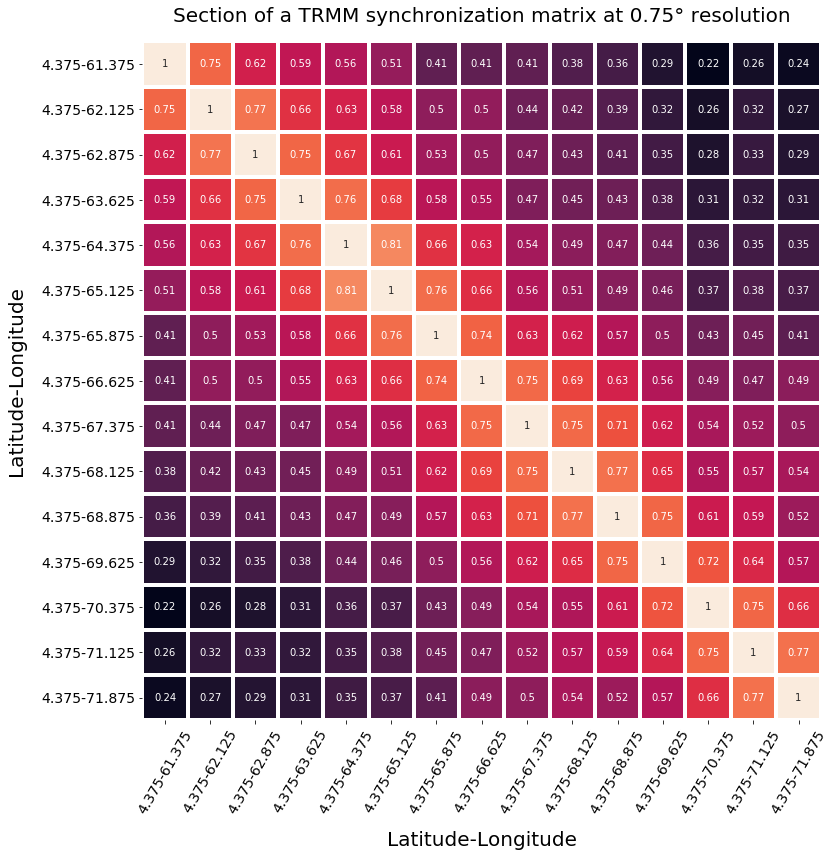
\includegraphics[width=0.65\textwidth]{./99_appendix/img/trmm_sync_example}
  \caption{Exemplary synchronization matrix for TRMM at a 0.75\degree resolution. We only show the top left 15x15 section of our actual matrix, as its full dimensions are 2401x2401 for a 0.75\degree resolution.}
  \label{fig:synchronization_matrix}
\end{figure}

Applying a numerical threshold to this synchronization matrix results in a matrix that contains only the most significantly synchronous values. Everything else is set to zero, including the diagonal of the matrix, as this would result in loops in the graph later on. Additionally, all elements above the threshold are set to one, yielding the adjacency matrix for an undirected, unweighted network (\cref{fig:adjacency_matrix}). \citet{Stolbova.2015} uses the 95th percentile for the threshold applied, as this removes all but the most statistically significant values.

\begin{figure}[h]
  \centering
  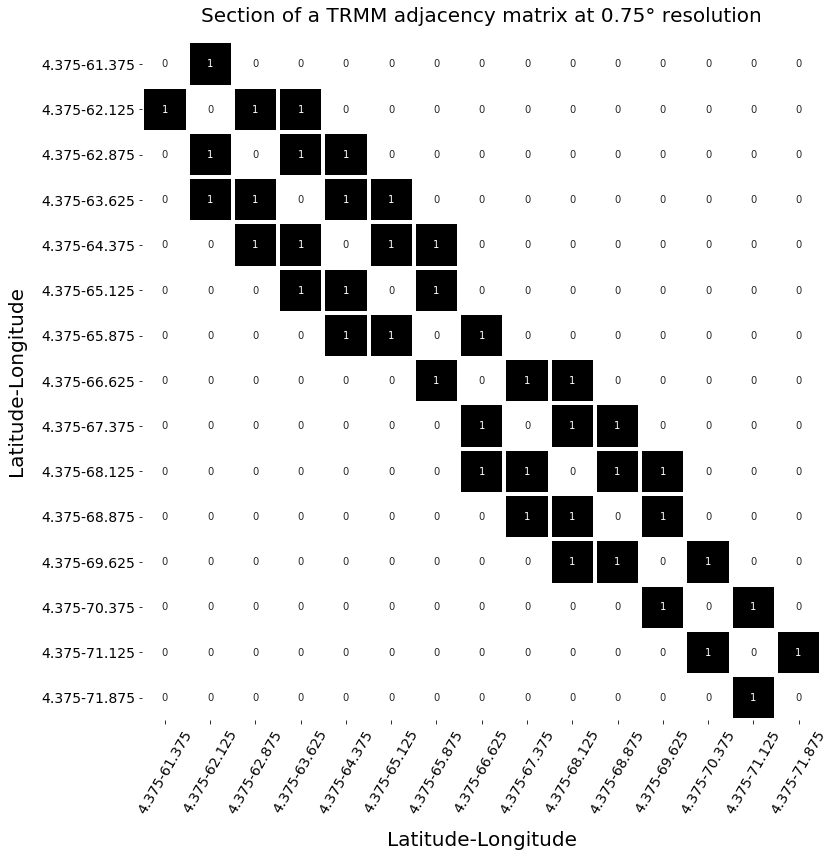
\includegraphics[width=0.65\textwidth]{./99_appendix/img/trmm_adjacency_example}
  \caption{Exemplary adjacency matrix for TRMM at a 0.75\degree resolution. We only show the top left 15x15 section of our actual matrix, as its full dimensions are 2401x2401 for a 0.75\degree resolution.}
  \label{fig:adjacency_matrix}
\end{figure}

Based upon the adjacency matrix, a network can then be computed and analyzed. However, before we detail our implementation of it, the next section briefly describes the measures that we will be using for said network analysis.

\subsection{Graph centrality}
\label{sst:network_measures}
Constructing climate networks from an adjacency matrix as seen in \cref{ssst:appl_climate_networks} enables the analysis of their structural features using various graph-based measures. We now shortly go over the concepts of the measures that we apply to our networks in this work.

The climate networks in \citet{Stolbova.2015} are analyzed using the \textit{degree} and \textit{betweenness} of nodes as well as using the \textit{average/maximal geographical link length} between them. We also base our analysis on the \textit{degree} and \textit{betweenness} measures but replace the link length calculations with the PageRank algorithm, which could, in our opinion, show more distinct patterns than the other two measures.

The \textit{degree} of a node in a network is quite simply defined as the amount of links that are connected to the respective node. The same holds for vertices in graphs and their connected edges.

Calculating the \textit{betweenness} or \textit{betweenness centrality} of a node is a more involved effort. A node has a high betweenness if a large portion of shortest paths in the network pass through the respective node. If the resulting betweenness is to be an exact measure, this basically necessitates the calculation of all shortest paths in the network, which gets increasingly complex with the size of the graph. There are, however, algorithms that achieve both accuracy and speed when calculating betweenness, one of the most popular being the approach proposed by \citet{Brandes.2001}\footnote{This algorithm is also used by the Python library \textit{networkx}, which we will be using for our calculations.}.

The final measure that we will apply to climate networks, the \textit{PageRank} algorithm, was originally developed and published by the founders of Google (amongst others), Larry Page and Sergey Brin, during their studies at Stanford University \citep{Page.1999}.

[TODO: finish page rank]

\section{Implementation}
\label{st:event_sync_implementation}
Our implementation of the event synchronization and climate network computations is strongly based on the concepts and measures as described in \cref{sst:event_sync} and \cref{sst:building_climate_network}. As our algorithmic implementation is most certainly different than the one used in the original work \citep{Stolbova.2015}, we shortly go over our approach to the problem in this section.

\subsection{Calculating event synchronization}
\label{sst:event_sync_calculation}

\subsubsection{Necessary preparations}
Before we are able to calculate the synchronicity for any two locations, the precipitation time series need to be transformed into series of events. Assume that we have extracted pre-monsoon time series as shown in \cref{tab:example_rainfall_ts} from the TRMM dataset and now want to convert these into extreme event series.

\begin{table}[h]
  \centering
  \begin{tabular}{ |c|c|ccccccc| }
    \hline
    Latitude & Longitude & 01.03.98 & ... & 29.05.98 & 30.05.98 & 31.05.98 & 01.03.99 & ...\\
    \hline
    13.375 & 67.375 & 0.0  & ... & 0.12 & 2.31  & 2.85  & 0.00 & ... \\
    16.375 & 91.375 & 0.0  & ... & 0.09 & 34.80 & 49.49 & 0.00 & ... \\
    34.375 & 67.375 & 0.52 & ... & 0.00 & 0.00  & 0.00  & 0.00 & ... \\
    34.375 & 88.375 & 0.86 & ... & 2.01 & 51.85 & 68.72 & 0.29 & ... \\
    \hline
  \end{tabular}
  \caption{Precipitation time series during pre-monsoon at 4 exemplary locations (TRMM, 0.75\degree).}
  \label{tab:example_rainfall_ts}
\end{table}

We calculate the 90th percentile seperately for each row and apply the result as a threshold to the respective row. This yields event series where each value represents the date of an extreme event in the series. This would look as shown in \cref{tab:example_rainfall_events} if applied to the time series in \cref{tab:example_rainfall_ts}.

\begin{table}[h]
  \centering
  \begin{tabular}{ |c|c|ccccccc| }
    \hline
    Latitude & Longitude & 1 & 2 & 3 & 4 & 5 & 6 & ... \\
    \hline
    13.375 & 67.375 & 07.04.98 & 31.05.98 & 08.05.99 & 12.05.99 & 13.05.99 & 15.05.99 & ... \\
    16.375 & 91.375 & 17.05.98 & 18.05.98 & 19.05.98 & 30.04.99 & 01.05.99 & 05.05.99 & ... \\
    34.375 & 67.375 & 03.03.98 & 29.03.98 & 02.04.98 & 03.04.98 & 09.04.98 & 22.04.98 & ... \\
    34.375 & 88.375 & 18.03.98 & 30.03.98 & 31.03.98 & 01.04.98 & 05.04.98 & 19.04.98 & ... \\
    \hline
  \end{tabular}
  \caption{First events in the pre-monsoon extreme event series at 4 exemplary locations (TRMM, 0.75\degree).}
  \label{tab:example_rainfall_events}
\end{table}

With a matrix of extreme events as shown in excerpt in \cref{tab:example_rainfall_events}, we then want to calculate the event synchronization for all pairs of locations. \cref{tab:example_empty_sync} shows the state of a preliminary synchronization matrix before running any of the calculations. Locations are always perfectly synchronous to themselves, leading to a diagonal that will always be filled with ones.

\begin{table}[h]
  \centering
  \begin{tabular}{ |cc|cccc| }
    \hline
     & Latitude & 13.375 & 16.375 & 34.375 & 34.375 \\
    Latitude & Longitude & 67.375 & 91.375 & 67.375 & 88.375 \\
    \hline
    13.375 & 67.375 & 1 &   &   &   \\
    16.375 & 91.375 &   & 1 &   &   \\
    34.375 & 67.375 &   &   & 1 &   \\
    34.375 & 88.375 &   &   &   & 1 \\
    \hline
  \end{tabular}
  \caption{Empty synchronization matrix for 4 exemplary locations (TRMM, 0.75\degree).}
  \label{tab:example_empty_sync}
\end{table}

To further fill in the values of the synchronization matrix in \cref{tab:example_empty_sync}, our algorithm only needs to perform calculations for one of the now empty halves of the matrix. This is due to the fact that, at least in our approach, the synchronization between two locations can be symmetrically applied to both their permutations. The original work on event synchronization by \citet{QuianQuiroga.2002} describes some asymmetrical measures, that were, however, not used in the work of \citet{Stolbova.2015}.

Going forward, we use \textit{unix timestamps}\footnote{Unix timestamps measure the number of seconds (without leap seconds) that have elapsed since the 01.01.1970 at 00:00 UTC. For example, "01.03.1998 00:00" would be represented as 888710400.} to represent dates instead of the full representation shown in the examples of this section, as they are much easier to process using mathematical formulas (but less intuitive to visualize).

\pagebreak
\subsubsection{Synchronization of two locations}
Having explained the necessary setup of the event synchronization algorithm, we now go over some of the concepts of our implementation. To calculate the synchronization between any two locations (i.e., \textit{location1} and \textit{location2}), we need to process both time series and compare each event in \textit{location1} to the appropriate events in \textit{location2}, taking the immediate neighbors of both locations into account.

We found that this naturally fits the description of a sliding window approach: a sliding window of size three over the event series of a location always encompasses a current event, its predecessor and its successor and thus everything we need for the time lag calculation. Application of a sliding window to \textit{location1} and nesting another such window for \textit{location2} then leads us to a naive implementation of the event synchronization algorithm as shown in \cref{lst:event_synchronization}.

\begin{listing}[H]
  \begin{minted}[mathescape,
    linenos,
    numbersep=5pt,
    gobble=4,
    frame=lines,
    framesep=2mm]{python}

    def calculate_synchronization(location1, location2):
        # initialize the number of synchronous events for the two locations
        num_sync_events = 0

        # iterate over all timesteps in location1 using a sliding window
        for i_prev, i_current, i_next in sliding_window(location1, 3):

            # iterate over all timesteps in location2 using a sliding window
            for j_prev, j_current, j_next in sliding_window(location2, 3):

                # calculate the time delta between the current events
                current_diff = i_current - j_current

                # check if the current events occur simultaneously
                if current_diff == 0:
                    num_sync_events += 0.5
                    continue

                # calculate the time lag based on the two sliding windows
                time_lag = 0.5 * min(
                    i_next - i_current, i_current - i_prev,
                    j_next - j_current, j_current - j_prev)

                # decide whether the events are synchronous
                if 0 < current_diff <= time_lag:
                    num_sync_events += 1.0

        return num_sync_events

  \end{minted}
  \caption{Python pseudocode for a simplified event synchronization algorithm, applicable to any two series of events.}
  \label{lst:event_synchronization}
\end{listing}

The event synchronization algorithm as described in \cref{lst:event_synchronization} results in the number of synchronous events between \textit{location1} and \textit{location2} where the event in \textit{location2} leads the event in \textit{location1}. This is, however, only part of the full synchronization synchronization calculation, as we also need the number of synchronous events where \textit{location1} leads \textit{location2}, i.e., we need to evaluate $calculate\_synchronization(location2, location1)$. This is the reason that simultaneous events only count as "half synchronous": they are counted in both these calculations and, in total, then result in one synchronous event.

Calculating the strength of synchronization then boils down to a simple application of formula \eqref{eq:sync_strength} from \pageref{eq:sync_strength} and is further presented in \cref{lst:sync_strength}.

\begin{listing}[H]
  \begin{minted}[mathescape,
    linenos,
    numbersep=5pt,
    gobble=4,
    frame=lines,
    framesep=2mm]{python}

    def calculate_sync_strength(loc1_events, loc2_events):
        # calculate synchronized events between loc1 and loc2 (and reverse)
        loc1_sync = calculate_synchronization(loc1_events, loc2_events)
        loc2_sync = calculate_synchronization(loc2_events, loc1_events)

        # calculate the strength of synchronization
        sync_strength = (loc1_sync + loc2_sync) / \
            math.sqrt((len(loc1_events) - 2) * (len(loc2_events) - 2))

        # return the strength of synchronization
        # and the total and separate numbers of synchronous events
        return sync_strength, loc1_sync + loc2_sync, loc1_sync, loc2_sync

  \end{minted}
  \caption{Python pseudocode for the calculation of the synchronization strength between any two series of events.}
  \label{lst:sync_strength}
\end{listing}

\subsubsection{Computing the values of the synchronization matrix}
We then make use of \cref{lst:sync_strength} to fill in the missing values in a synchronization matrix like the one we have already prepared (see \cref{tab:example_empty_sync}). Firstly, the algorithm is applied to each empty cell in the upper half of the matrix, yielding a triangular matrix. Secondly, as the synchronization strength measure is symmetrical, the lower half of the matrix is filled by simply mirroring the upper half. This yields two matrices: one containing the synchronization strength and one containing the total count of synchronous events for all pairs of locations. A third asymmetrical matrix seperately contains the number of events where $i$ leads $j$ as well as the number of events where $j$ leads $i$. The procedure is shown in detail in \cref{lst:sync_matrix}.

\begin{listing}[H]
  \begin{minted}[mathescape,
    linenos,
    numbersep=5pt,
    gobble=4,
    frame=lines,
    framesep=2mm]{python}

    def calculate_sync_matrix(event_matrix):
        # calculate the sync strength for each permutation of grid cells
        for i in range(0, sync_matrix.shape[0]):
            # as the matrix is symmetrical, only calculate the upper half
            for j in range(0, i + 1):
                # calculate the synchronicity for the permutation of rows
                sync_strength, count = calculate_sync_strength(
                    event_matrix[i], event_matrix[j])

                # save results in the respective matrices
                sync_matrix[i, j] = sync_strength
                sync_matrix[j, i] = sync_strength
                count_matrix[i, j] = count
                count_matrix[j, i] = count
                directed_matrix[i, j] = i_leads
                directed_matrix[j, i] = j_leads

        return sync_matrix, count_matrix, directed_matrix

  \end{minted}
  \caption{Python pseudocode for processing an entire event matrix.}
  \label{lst:sync_matrix}
\end{listing}

\subsubsection{Improvements for the event synchronization algorithm}
The implementation as shown so far naively processes all possible combinations of events when calculating the event synchronization measure. Given $i$ events at \textit{location1} and $j$ events at \textit{location2}, the simple nested loop algorithm potentially calculates a time lag up to $i * j$ times. This results in a lot of wasted computation, because the actual portion of $j$ that can be synchronous tends to be very small.

\begin{listing}[H]
  \begin{minted}[mathescape,
    linenos,
    numbersep=5pt,
    gobble=4,
    frame=lines,
    framesep=2mm]{python}

    def calculate_synchronization(location1, location2):
        # initialize the number of synchronous events for the two locations
        num_sync_events = 0

        # iterate over all timesteps in location1 using a sliding window
        for i_prev, i_current, i_next in sliding_window(location1, 3):
            # calculate the last timestamp of location2 that could be synchronous
            latest = i_current + 0.5 * min(i_current - i_prev, i_next - i_current)

            # iterate over all timesteps in location2 using a sliding window
            for j_prev, j_current, j_next in sliding_window(location2, 3):
                # continue for timestamps that cannot possibly be synchronous
                if j_current < earliest:
                    continue

                # if the difference gets negative, continue
                # the second pass will encompass these combinations
                if current_diff < 0:
                    continue

                # check if the events occur simultaneously
                if current_diff == 0:
                    num_sync_events += 0.5
                    continue

                # break for timestamps that cannot possibly be synchronous
                # i.e. are much too late
                if j_current > latest:
                    break

                # calculate the time lag based on the two sliding windows
                time_lag = 0.5 * min(
                    i_next - i_current, i_current - i_prev,
                    j_next - j_current, j_current - j_prev)

                # decide whether the events are synchronous
                if 0 < current_diff <= time_lag:
                    num_sync_events += 1.0

        return num_sync_events

  \end{minted}
  \caption{Python pseudocode for an improved version of the event synchronization algorithm, applicable to any two series of events.}
  \label{lst:event_synchronization_improved}
\end{listing}

However, we can define a range of events in $j$ for which we are sure that they cannot be synchronous and skip their evaluation (see an improved version of the algorithm in \cref{lst:event_synchronization_improved}). According to our implementation, this holds for two cases: firstly, if the event in $j$ occurs at earlier than the event in $i$, it can be safely skipped, as the reversed iteration of the algorithm will deal with it. Secondly, an event in $j$ can also be skipped if the event in $j$ occurs later than the time lag of the event in $i$. Additionally, we can safely break the inner loop early, as further events in $j$ only occur even later.

Notice that another (obvious) improvement would be to "simply filter" the \textit{location2} series such that it only contains the few events that need to be evaluated, after which no more breaking or skipping in the loop would be needed. However, upon evaluation of such an approach, it became clear that this is not necessarily faster. Adequately filtering the series $j$ necessitates some complex indexing and selection operations, which in turn depend on the existence of an index or hash table for $j$. Creating such indices can take more than a second for a single series, making the approach especially slow for large matrices.

\subsection{Building climate networks}
\label{sst:building_climate_network}
Based on \cref{ssst:appl_climate_networks}, the next step after the computation of a full event synchronization matrix is the transformation of said matrix into an adjacency matrix, allowing the creation of a network and its analysis using various methods and libraries. This transformation is a simple thresholding of the matrix using a specified percentile.

\citet{Stolbova.2015} uses the 95th percentile to threshold the adjacency matrix, leaving only the most statistically significant links in the network. However, we use an aggregated {0.75\degree} resolution for our base dataset (instead of the full {0.25\degree} resolution), meaning that there is already much less data available to analyze (but the data is also less sparse). We thus use a decreased threshold equal to the 90th percentile.

We further expand upon the work of \citet{Stolbova.2015} by building weighted networks in addition to the unweighted networks that have already been explored. To build a weighted network, values above the threshold are left as is, leading to links that are weighted with their corresponding synchronization measure. Contrarily, all values above the threshold are uniformly set to one when building an unweighted network.

The creation of a climate network based on an adjacency network, as well as the calculation of the degree, betweenness and PageRank for all nodes in the network, are a matter of a few lines of code as shown in \cref{lst:climate_networks}.

\begin{listing}[H]
  \begin{minted}[mathescape,
    linenos,
    numbersep=5pt,
    gobble=4,
    frame=lines,
    framesep=2mm]{python}

    # build a graph from an adjacency matrix
    # using the networkx (nx) Python library
    graph = nx.from_numpy_matrix(adjacency_matrix)

    # calculate the degree, betweenness and PageRank for all nodes
    # the weighted variant (simply leave the parameter for the unweighted variant)
    nodes_degree = graph.degree(weight='weight')
    nodes_betweenness = nx.betweenness_centrality(graph, normalized=False, weight='weight')
    nodes_pagerank = nx.pagerank_numpy(graph, weight='weight')

  \end{minted}
  \caption{Simplified Python pseudocode for the creation of a climate network from an adjacency matrix as well as the calculation of corresponding network measures.}
  \label{lst:climate_networks}
\end{listing}

The results of applying the algorithms we have described in this section to the TRMM dataset, more specifically the pre-monsoon, monsoon and post-monsoon seasons as extracted from TRMM, are presented in the next section (\cref{st:event_sync_results}).

\section{Results \& Evaluation}
\label{st:event_sync_results}


\subsection{Dataset}
Our results are based on the TRMM dataset as introduced in \cref{sst:trmm_dataset}. We have extracted data for the years 1998-2016, which corresponds to all years that were fully available at the time. The area included in the dataset was cropped to an extended overview over the Indian subcontinent, more specifically the area between 4.125-40.625N, 61.125-97.625E. Aggregation of the native {0.25\degree} resolution to a lower {0.75\degree} resolution then yields grid borders of 4.375-40.375N, 61.375-97.375E \footnote{The TRMM dataset needed to be aggregated to reduce the computational effort required for event synchronization and climate network calculations. Going from {0.25\degree} to {0.75\degree} resolution effectively reduced the size of event synchronization matrices from 21609x21609 to around 2401x2401 (81x).}.

\subsection{Pre-monsoon season (MAM)}
The results of applying our algorithms to the pre-monsoon season, namely the months of March, April and May (MAM), are shown in \cref{fig:results_mam}. We show the unweighted version, as also computed in \citet{Stolbova.2015}, as well as our extended version with weights applied to the edges in the network. To enable intercomparison with the work of \citet{Stolbova.2015}, which this part of our work is based on, we additionally assign the area identifiers used in her work to any areas we refer to.

The degree is strongest over the Indian ocean, enframing the Indian subcontinent from both east and west. On the western side lies the Arabian Sea, over which an area of high degree extends from the far west up to the natural barrier of the Western Ghats mountain range (WG). A similar but smaller area over the Bay of Bengal to the east of the Indian subcontinent ranges from the Indian coast onto the lands of Myanmar (BoB). Further patches of significant degree can be found over the Tibetan Plateau (TP), over north-eastern India and Nepal at the brim of the Himalayas (Himalayas) and over areas of Pakistan and Afghanistan (NP, representing North-Pakistan).

The patterns in the betweenness are much less clear and conclusive. There are, however, still spots that display significantly high betweenness, especially the area over Nepal (Himalayas). Additionally, smaller patches of high betweenness are sprinkled over the Tibetan Plateau (TP), to the north of Pakistan and over central India.

Looking at the PageRank analysis of our climate networks, a similarity with the degree is immediately obvious. PageRank closely follows the stronger patterns we have seen when analyzing the degree. However, PageRank  also [TODO: updated PageRank]

Comparison of the unweighted and weighted visualizations shows little difference. The main patterns are the same and differ only in the pronounciation of details.

\begin{figure}[h]
  \centering
  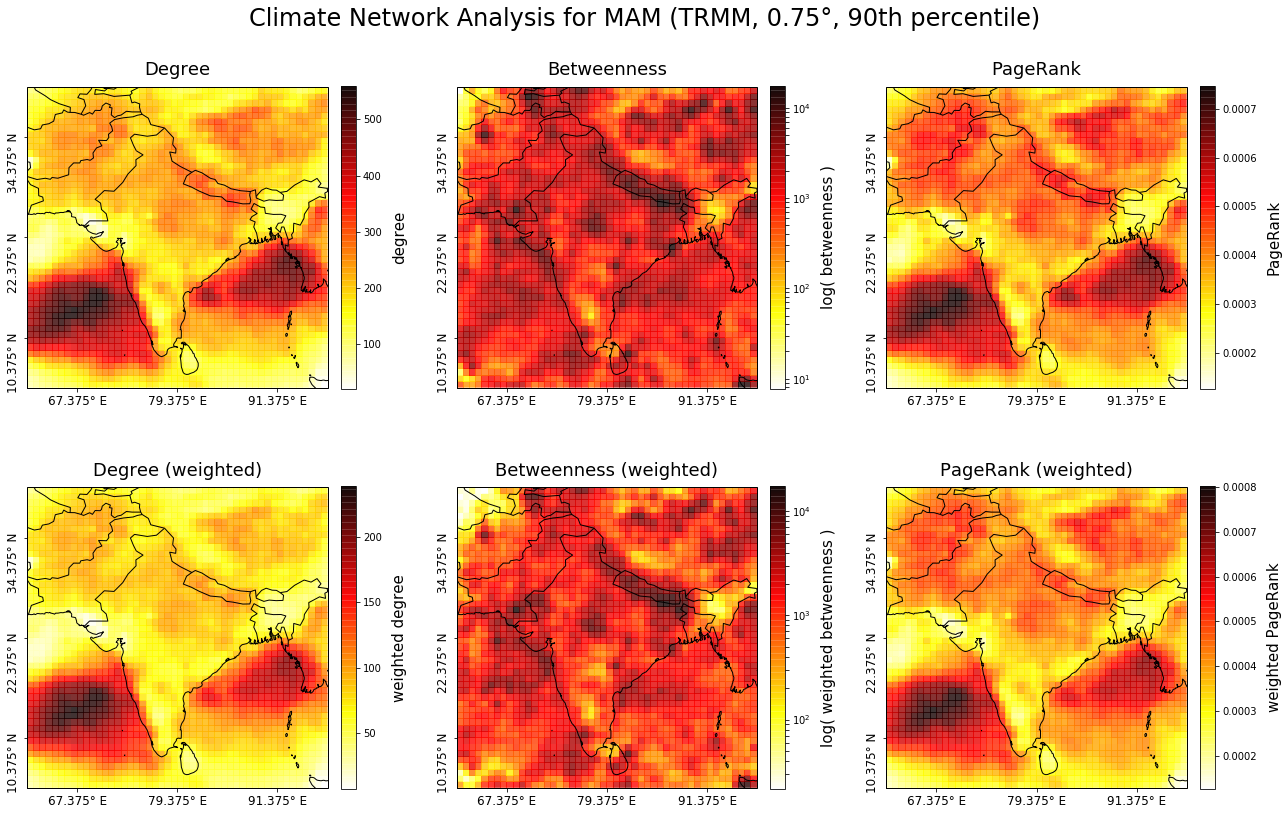
\includegraphics[width=\textwidth]{{./99_appendix/img/event_sync_0.75-0.9_MAM}.png}
  \caption{Weighted and unweighted degree, betweenness and PageRank for the pre-monsoon season (MAM). Based on the TRMM dataset at {0.75\degree} resolution.}
  \label{fig:results_mam}
\end{figure}


[TODO: interpret the results, incorporating knowledge of impacting factors]

[TODO: compare with Stolbova]


\subsection{Monsoon season (JJAS)}
Analyzing the months of the primary monsoon season (JJAS, June-September) as shown in \cref{fig:results_jjas} yields somewhat unexpected results: degree and betweenness both display a strong but compact pattern over Northern Pakistan (NP). Further areas of significant degree are located on the Tibetan Plateau (TB) and over the Indian Ocean around the southern tip of India (Arabian Sea/WG and BoB). High betweenness can be seen near the Western Ghats (WG) and Kerala as well as on the other side of the southern tip of India.

\begin{figure}[h]
  \centering
  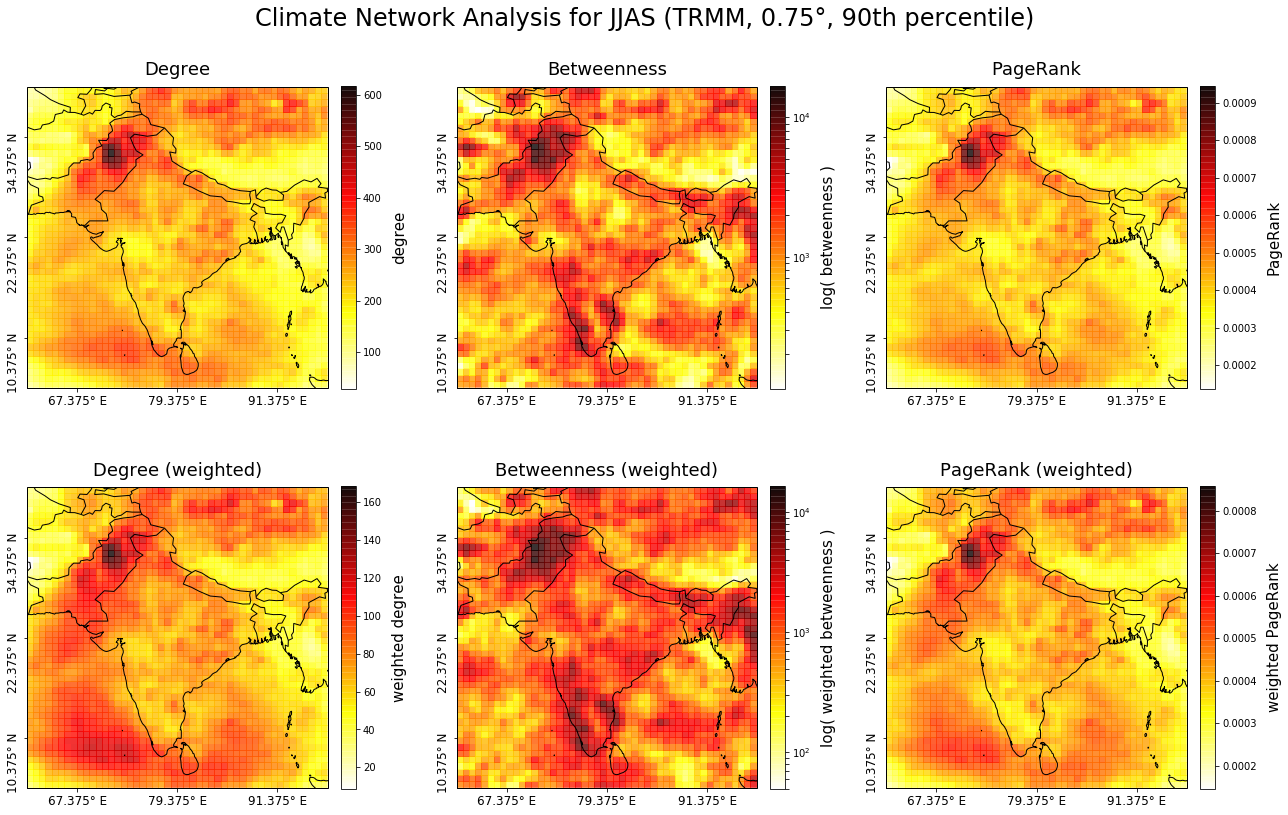
\includegraphics[width=\textwidth]{{./99_appendix/img/event_sync_0.75-0.9_JJAS}.png}
  \caption{Weighted and unweighted degree, betweenness and PageRank for the primary monsoon season (JJAS). Based on the TRMM dataset at {0.75\degree} resolution.}
  \label{fig:results_jjas}
\end{figure}


[TODO: interpret the results, incorporating knowledge of impacting factors]

[TODO: compare with Stolbova]


\subsection{Post-monsoon season (OND)}
The post-monsoon season (OND, October-December) is typically also called the north-east monsoon. The reason for this is clearly identifiable based on the network measures this season exhibits. A single area of very high degree encompasses entire central and north-eastern India, starting over the Arabian Sea (WG) and ranging well into Bangladesh. The degree in this area is at its highest close to the Himalayas on the Nepali border. The area further extends over the Tibetan Plateau (TP), although with less strength.



\begin{figure}[h]
  \centering
  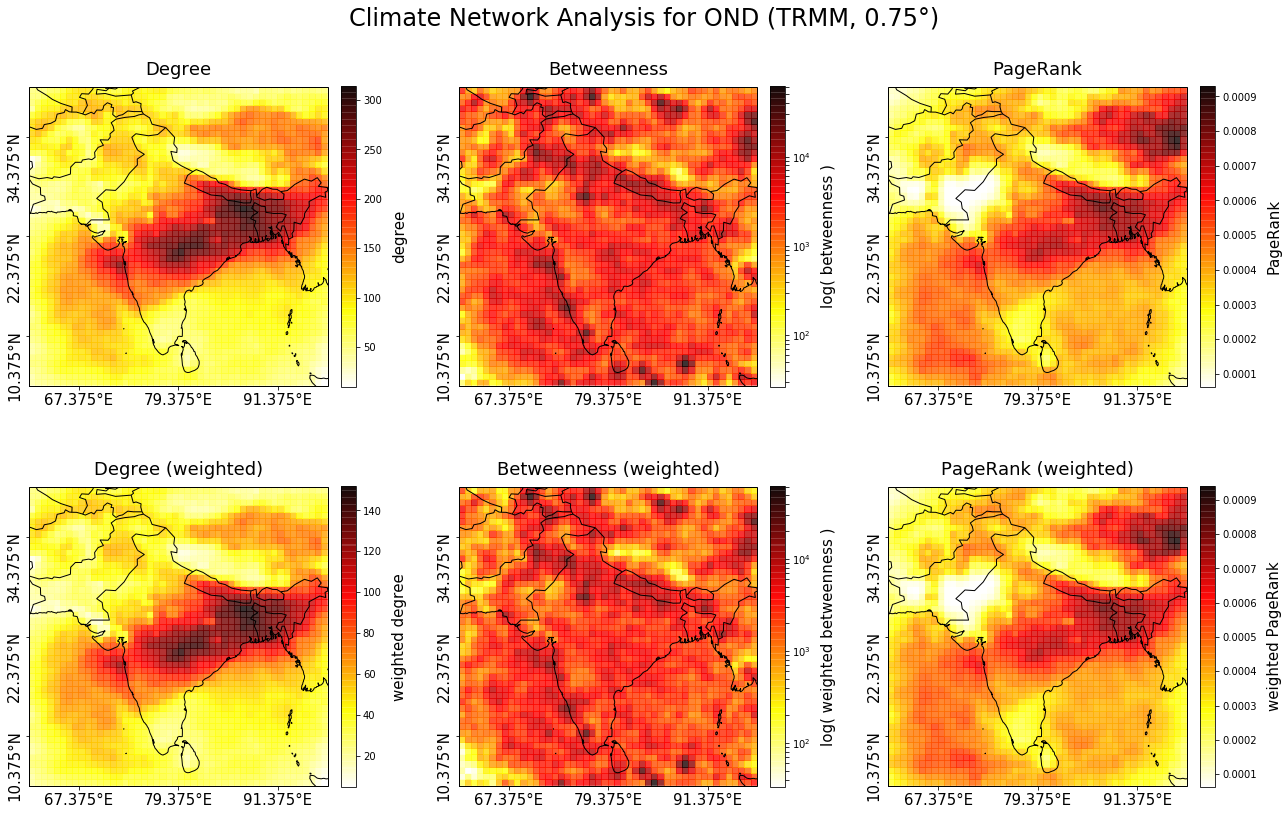
\includegraphics[width=\textwidth]{{./99_appendix/img/event_sync_0.75-0.9_OND}.png}
  \caption{Weighted and unweighted degree, betweenness and PageRank for the post-monsoon season (OND). Based on the TRMM dataset at {0.75\degree} resolution.}
  \label{fig:results_ond}
\end{figure}





[TODO: interpret the results, incorporating knowledge of impacting factors]

[TODO: compare with Stolbova]



\section{Conclusion}
\label{st:event_sync_conclusion}
[TODO: conclude the chapter]
